% ----------------------------------------------------------------------------
% Apresentação
% ----------------------------------------------------------------------------
 
\chapter{Apresentação}

Pure Data é um ambiente visual de programação musical que permite a criação de
aplicações musicais complexas a partir da combinação de componentes visuais
mais simples chamados \textbf{objetos}. As distribuições oficiais do Pure Data
contêm diversos objetos prontos para o uso, mas também permitem a extensão de
suas funcionalidades através da criação de novos objetos utilizando C/C++.
Desta forma, novas linhas de código escritas pelo usuário são compilados como
bibliotecas dinâmicas e podem ser carregadas pelo programa em tempo de
execução. Objetos desta forma levam o nome de \textbf{\\externals}.

Este é um tutorial prático para o desenvolvimento de \externals em C para o
Pure Data. A iniciativa de escrever este documento surgiu no primeiro semestre
de 2011, durante a disciplina de Computação Musical ministrada pelo professor
Marcelo Gomes de Queiroz no Instituto de Matemática e Estatística da
Universidade de São Paulo. A intenção deste tutorial é auxiliar programadores
a desenvolver \externals de maneira bastante simples através de exemplos
práticos.

Mais do que ampliar a gama de objetos do Pure Data e criar novos objetos, o
objetivo deste trabalho é também fornecer ao pesquisador de computação musical
uma ferramenta para implementar e testar algoritmos de processamento de áudio
para caráter de estudo. Isto significa que podemos reimplementar várias coisas
que já existem no Pure Data simplesmente porque é didático programar e colocar
algoritmos para funcionar.

\section{Escrevendo \externals}

O código fonte do Pure Data é organizado de acordo com convenções de
programação orientada a objetos. Para o desenvolvimento de \externals, é
necessário seguir estas convenções e fornecer ao ambiente uma nova classe com
alguns métodos específicos, como veremos mais adiante.

Para desenvolver para o Pure Data, é necessário importar a biblioteca
m\_pd.h\footnote{Disponível em
http://compbio.cs.toronto.edu/repos/snowflock/mpich-1.2.7/mpid/mpd/mpd.h}. Há
um tutorial para escrever \externals feito pelo IOHannes, um dos programadores
do Pure Data\footnote{Disponível em
http://iem.at/pd/externals-HOWTO/pd-externals-HOWTO.pdf}. Apesar deste
documento ter sido meu ponto de partida, boa parte do que contém no presente
tutorial foi aprendido lendo o código-fonte de \externals do repositório do
próprio Pure Data
(http://pure-data.svn.sourceforge.net/viewvc/pure-data/trunk/\externals/).

\section{Organizando seus \externals}

É praxe que o arquivo do \external tenha o mesmo nome que o \external. Se
fossemos fazer, por exemplo, um trigger, o mesmo estaria em um arquivo chamado
trigger.c e seria compilado em um \external chamado trigger.pd\_linux ou
trigger.dll ou trigger.pd\_irix5 ou trigger.pd\_darwin. Isto não é obrigatório
mas é uma convenção que facilita a busca do código-fonte deste \external no
repositório.

\section{Compilando seus \externals}

Um \external precisa ser compilado e depois linkado como \external. A versão
Linux pode ser feita com os comandos:

\begin{lstlisting}
cc -DPD -O2 -fPIC -funroll-loops -fomit-frame-pointer 
	-Wall -W -Wshadow -Wstrict-prototypes -Werror 
	-Wno-unused -Wno-parentheses -Wno-switch 
	-o example1.o -c example1.c
ld -export_dynamic  -shared -o example1.pd_linux 
	example1.o -lc -lm
rm example1.o
\end{lstlisting}

Para compilar, o ideal é criarmos um Makefile. Todas as pastas de exemplos
deste tutorial estão acompanhadas de um makefile feito pelo Marcelo Queiroz.

\section{Criando help para seus \externals}

O arquivo de help deve ter o mesmo nome que o \external. Por exemplo, para o
exemplo1.c com o objeto exemplo1 temos o arquivo example1-help.pd. Este
arquivo do Pure Data com exemplo deve acompanhar o \external na instalação,
ficando na mesma pasta que o \external compilado.  Há a possibilidade de
associarmos a cada \external outros arquivos que não sigam esta convenção e a
mesma será apresentada no próximo capítulo.

\section{Executando seu \external}

Se você executar o Pure Data na mesma pasta aonde está seu \external compilado,
o mesmo irá funcionar. Caso não esteja executando o Pure Data via terminal
deverá colocar a pasta aonde o \external se encontra no caminho de busca do
Pure Data.

\begin{figure}[h!]
	\centering
	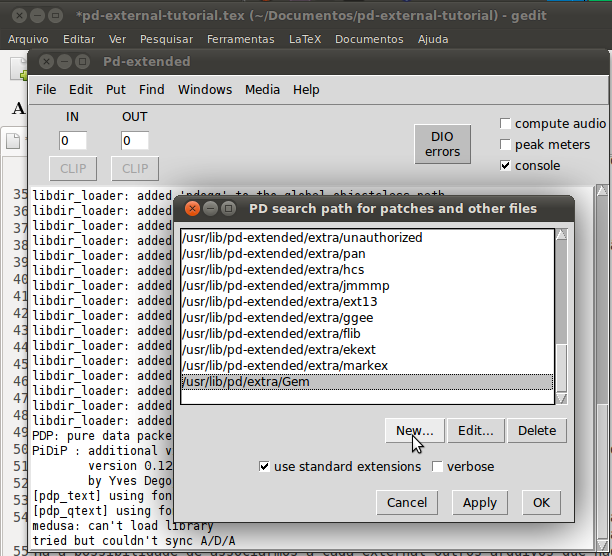
\includegraphics[width=0.7\textwidth]{path}
	\caption{Adicionando o diretório do seu \external no Pure Data.}
\end{figure}

Para carregar uma biblioteca de \externals (mais de um \external no mesmo
arquivo-fonte), é necessário adicionar a biblioteca no Pure Data:

\begin{lstlisting}
pdextended  -lib medusa medusa-help.pd 
\end{lstlisting}

Ou 

\begin{figure}[h!]
	\centering
	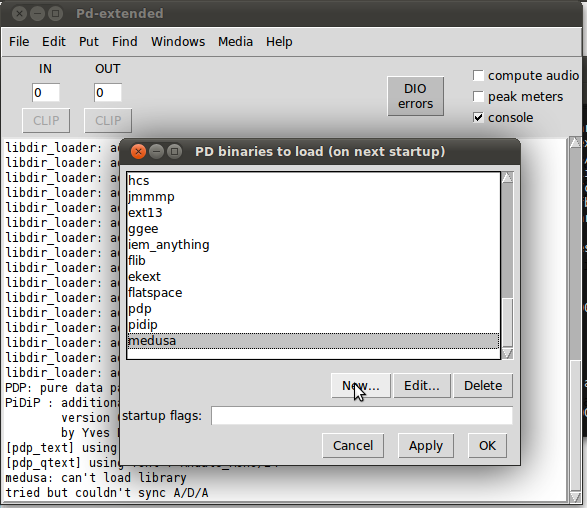
\includegraphics[width=0.7\textwidth]{startup}
	\caption{Adicionando sua biblioteca no Pure Data.}
\end{figure}


